\documentclass[10pt,ignorenonframetext,]{beamer}
\setbeamertemplate{caption}[numbered]
\setbeamertemplate{caption label separator}{: }
\setbeamercolor{caption name}{fg=normal text.fg}
\beamertemplatenavigationsymbolsempty
\usepackage{lmodern}
\usepackage{amssymb,amsmath}
\usepackage{ifxetex,ifluatex}
\usepackage{fixltx2e} % provides \textsubscript
\ifnum 0\ifxetex 1\fi\ifluatex 1\fi=0 % if pdftex
  \usepackage[T1]{fontenc}
  \usepackage[utf8]{inputenc}
\else % if luatex or xelatex
  \ifxetex
    \usepackage{mathspec}
  \else
    \usepackage{fontspec}
  \fi
  \defaultfontfeatures{Ligatures=TeX,Scale=MatchLowercase}
\fi
% use upquote if available, for straight quotes in verbatim environments
\IfFileExists{upquote.sty}{\usepackage{upquote}}{}
% use microtype if available
\IfFileExists{microtype.sty}{%
\usepackage{microtype}
\UseMicrotypeSet[protrusion]{basicmath} % disable protrusion for tt fonts
}{}
\newif\ifbibliography
\hypersetup{
            pdftitle={Modélisation statistique},
            pdfauthor={Marie-Pierre Etienne},
            pdfborder={0 0 0},
            breaklinks=true}
\urlstyle{same}  % don't use monospace font for urls
\usepackage{color}
\usepackage{fancyvrb}
\newcommand{\VerbBar}{|}
\newcommand{\VERB}{\Verb[commandchars=\\\{\}]}
\DefineVerbatimEnvironment{Highlighting}{Verbatim}{commandchars=\\\{\}}
% Add ',fontsize=\small' for more characters per line
\usepackage{framed}
\definecolor{shadecolor}{RGB}{248,248,248}
\newenvironment{Shaded}{\begin{snugshade}}{\end{snugshade}}
\newcommand{\KeywordTok}[1]{\textcolor[rgb]{0.13,0.29,0.53}{\textbf{#1}}}
\newcommand{\DataTypeTok}[1]{\textcolor[rgb]{0.13,0.29,0.53}{#1}}
\newcommand{\DecValTok}[1]{\textcolor[rgb]{0.00,0.00,0.81}{#1}}
\newcommand{\BaseNTok}[1]{\textcolor[rgb]{0.00,0.00,0.81}{#1}}
\newcommand{\FloatTok}[1]{\textcolor[rgb]{0.00,0.00,0.81}{#1}}
\newcommand{\ConstantTok}[1]{\textcolor[rgb]{0.00,0.00,0.00}{#1}}
\newcommand{\CharTok}[1]{\textcolor[rgb]{0.31,0.60,0.02}{#1}}
\newcommand{\SpecialCharTok}[1]{\textcolor[rgb]{0.00,0.00,0.00}{#1}}
\newcommand{\StringTok}[1]{\textcolor[rgb]{0.31,0.60,0.02}{#1}}
\newcommand{\VerbatimStringTok}[1]{\textcolor[rgb]{0.31,0.60,0.02}{#1}}
\newcommand{\SpecialStringTok}[1]{\textcolor[rgb]{0.31,0.60,0.02}{#1}}
\newcommand{\ImportTok}[1]{#1}
\newcommand{\CommentTok}[1]{\textcolor[rgb]{0.56,0.35,0.01}{\textit{#1}}}
\newcommand{\DocumentationTok}[1]{\textcolor[rgb]{0.56,0.35,0.01}{\textbf{\textit{#1}}}}
\newcommand{\AnnotationTok}[1]{\textcolor[rgb]{0.56,0.35,0.01}{\textbf{\textit{#1}}}}
\newcommand{\CommentVarTok}[1]{\textcolor[rgb]{0.56,0.35,0.01}{\textbf{\textit{#1}}}}
\newcommand{\OtherTok}[1]{\textcolor[rgb]{0.56,0.35,0.01}{#1}}
\newcommand{\FunctionTok}[1]{\textcolor[rgb]{0.00,0.00,0.00}{#1}}
\newcommand{\VariableTok}[1]{\textcolor[rgb]{0.00,0.00,0.00}{#1}}
\newcommand{\ControlFlowTok}[1]{\textcolor[rgb]{0.13,0.29,0.53}{\textbf{#1}}}
\newcommand{\OperatorTok}[1]{\textcolor[rgb]{0.81,0.36,0.00}{\textbf{#1}}}
\newcommand{\BuiltInTok}[1]{#1}
\newcommand{\ExtensionTok}[1]{#1}
\newcommand{\PreprocessorTok}[1]{\textcolor[rgb]{0.56,0.35,0.01}{\textit{#1}}}
\newcommand{\AttributeTok}[1]{\textcolor[rgb]{0.77,0.63,0.00}{#1}}
\newcommand{\RegionMarkerTok}[1]{#1}
\newcommand{\InformationTok}[1]{\textcolor[rgb]{0.56,0.35,0.01}{\textbf{\textit{#1}}}}
\newcommand{\WarningTok}[1]{\textcolor[rgb]{0.56,0.35,0.01}{\textbf{\textit{#1}}}}
\newcommand{\AlertTok}[1]{\textcolor[rgb]{0.94,0.16,0.16}{#1}}
\newcommand{\ErrorTok}[1]{\textcolor[rgb]{0.64,0.00,0.00}{\textbf{#1}}}
\newcommand{\NormalTok}[1]{#1}
\usepackage{graphicx,grffile}
\makeatletter
\def\maxwidth{\ifdim\Gin@nat@width>\linewidth\linewidth\else\Gin@nat@width\fi}
\def\maxheight{\ifdim\Gin@nat@height>\textheight0.8\textheight\else\Gin@nat@height\fi}
\makeatother
% Scale images if necessary, so that they will not overflow the page
% margins by default, and it is still possible to overwrite the defaults
% using explicit options in \includegraphics[width, height, ...]{}
\setkeys{Gin}{width=\maxwidth,height=\maxheight,keepaspectratio}

% Prevent slide breaks in the middle of a paragraph:
\widowpenalties 1 10000
\raggedbottom

\AtBeginPart{
  \let\insertpartnumber\relax
  \let\partname\relax
  \frame{\partpage}
}
\AtBeginSection{
  \ifbibliography
  \else
    \let\insertsectionnumber\relax
    \let\sectionname\relax
    \frame{\sectionpage}
  \fi
}
\AtBeginSubsection{
  \let\insertsubsectionnumber\relax
  \let\subsectionname\relax
  \frame{\subsectionpage}
}

\setlength{\parindent}{0pt}
\setlength{\parskip}{6pt plus 2pt minus 1pt}
\setlength{\emergencystretch}{3em}  % prevent overfull lines
\providecommand{\tightlist}{%
  \setlength{\itemsep}{0pt}\setlength{\parskip}{0pt}}
\setcounter{secnumdepth}{0}
\usepackage{../resources/themeBeamer}

\usepackage{framed,xcolor}
\usepackage{etextools}


%%%%%%%%%%%%%%%%%%%%%%
%%% color
\definecolor{monvert}{RGB}{0,153,0}
\definecolor{orange}{HTML}{C5A61A}
\definecolor{orangepale}{HTML}{FFBA62}
\definecolor{orangetrespale}{rgb}{1,0.9,0.68}
\definecolor{vertfonce}{HTML}{22C25A}
\definecolor{rougefonce}{HTML}{EC1C35}
\definecolor{jolibleu}{HTML}{317589}
\definecolor{jolibleufonce}{HTML}{628B9F}
\definecolor{grisclair}{HTML}{F9FBFC}
\definecolor{bleu}{HTML}{598DE2}



% make space after console-output smaller:
\setlength{\OuterFrameSep}{2pt}
\makeatletter
\preto{\@verbatim}{\topsep=0pt \partopsep=0pt }
\makeatother

\makeatletter
\addtobeamertemplate{block begin}{
\def\@listi{\leftmargin\leftmargini
              \topsep    0pt
              \parsep    0pt
              \itemsep   3pt plus 2pt minus 3pt}
\partopsep 0pt
}
\makeatother

\graphicspath{{../resources/common_figs/}}
\usepackage{tikz}
\usetikzlibrary{calc,shapes,backgrounds,arrows,automata,shadows,positioning}
\tikzstyle{every state}=[fill=red,draw=none,scale=0.7,font=\small,text=white]
\tikzstyle{every edge}=[-,shorten >=1pt,auto,thin,draw]
\tikzstyle{alertstate}=[fill=bleu]
\definecolor{genecolor}{RGB}{94,135,173}

\let\oldtitle\title
\subtitle{\huge\oldtitle\normalsize}
\title{\currentCourse}
\institute{\currentInstitute}

\date{\currentDate}

\AtBeginSection{
  \begin{frame}<beamer>
    \frametitle{Outline}
    \framesubtitle{\insertpart}
    \tableofcontents[currentsection,currentsubsection, subsectionstyle=show/shaded/hide]  
  \end{frame}
}

\AtBeginSubsection{
  \begin{frame}<beamer>
    \frametitle{Outline}
    \framesubtitle{\insertpart}
    \tableofcontents[currentsection,currentsubsection, subsectionstyle=show/shaded/hide]  
  \end{frame}
}

\AtBeginSubsubsection{
  \begin{frame}<beamer>
    \frametitle{Outline}
    \framesubtitle{\insertpart}
    \tableofcontents[currentsection,currentsubsection, subsectionstyle=show/shaded/hide]  
  \end{frame}
}

\let\oldtitlepage\titlepage
\renewcommand{\titlepage}{%
    \oldtitlepage
    \vfill

\begin{tikzpicture}[remember picture,overlay]
  \node [xshift=2cm,yshift=1.5cm] at (current page.south west)    {
\includegraphics[width=2.5cm]{logo_dauphine}};
  \node [yshift=-3.5cm] at (current page.center)    {
\includegraphics[width=2cm]{sticker_sotr}};
  \node [xshift=-2cm,yshift=1.35cm] at (current page.south east)   {
\includegraphics[width=2.5cm]{logo_inra}};
\end{tikzpicture}
}

\title{Modélisation statistique}
\author{Marie-Pierre Etienne}
\institute{\url{https://github.com/MarieEtienne}}
\date{Septembre 2018}

\begin{document}
\frame{\titlepage}

\begin{frame}
  \frametitle{Outline}
  \tableofcontents[currentsection, sectionstyle=show/show,subsectionstyle=hide]
\end{frame}

\section{Introduction}\label{introduction}

\begin{frame}{Motivations}

\begin{itemize}
\tightlist
\item
  \textbf{Comprendre} : des mécanismes biologiques, économiques,
  \ldots{}
\end{itemize}

\end{frame}

\begin{frame}{Motivations}

\begin{itemize}
\tightlist
\item
  \textbf{Comprendre} : des mécanismes biologiques, économiques,
  \ldots{}
\end{itemize}

\includegraphics[width=2.08333in]{figures/LePape_al.png}
\includegraphics[width=1.04167in]{figures/LePape_al2.png}

Type de modèles :

~\includegraphics[width=1.56250in]{figures/LePape_al3.png}

\end{frame}

\begin{frame}{Motivations}

\begin{itemize}
\item
  \textbf{Comprendre} : des mécanismes biologiques, économiques,
  \ldots{}
\item
  \textbf{Prédire} : des tendances, des choix, \ldots{}.
\end{itemize}

\end{frame}

\begin{frame}{Motivations}

\begin{itemize}
\item
  \textbf{Comprendre} : des mécanismes biologiques, économiques,
  \ldots{}
\item
  \textbf{Prédire} : des tendances, des choix, \ldots{}.
\end{itemize}

~\includegraphics[width=2.08333in]{figures/iotc.png}

\end{frame}

\begin{frame}{Motivations}

\begin{itemize}
\item
  \textbf{Comprendre} : des mécanismes biologiques, économiques,
  \ldots{}
\item
  \textbf{Prédire} : des tendances, des choix, \ldots{}.
\item
  \textbf{Communiquer} : sur l'état d'un système, les conséquences d'une
  décision
\end{itemize}

\includegraphics[width=2.08333in]{figures/icatt_0.png}
\includegraphics[width=2.08333in]{figures/icatt.png}

\end{frame}

\begin{frame}{Les outils : différents types de modèles}

\begin{itemize}
\item
  \textbf{Machine Learning} (deep learning)\\
  \includegraphics[width=2.08333in]{figures/Deeplearning.png} Modèles
  boites noires, gourmands en données avec un but purement prédictif
  (réseaux de neurones, forêts aléatoires, \ldots{})
\item
  \textbf{Modèle stochastique}
\end{itemize}

De la simple mesure de corrélation jusqu'au modèle mécaniste \ldots{}.

\begin{itemize}
\tightlist
\item
  \textbf{Modèle déterministe}
\end{itemize}

Le plus souvent dans la panoplie des modèles mécanistes

\end{frame}

\begin{frame}{Un exemple : relation von Bertalanffy}

Des données de croisance \scriptsize

\begin{center}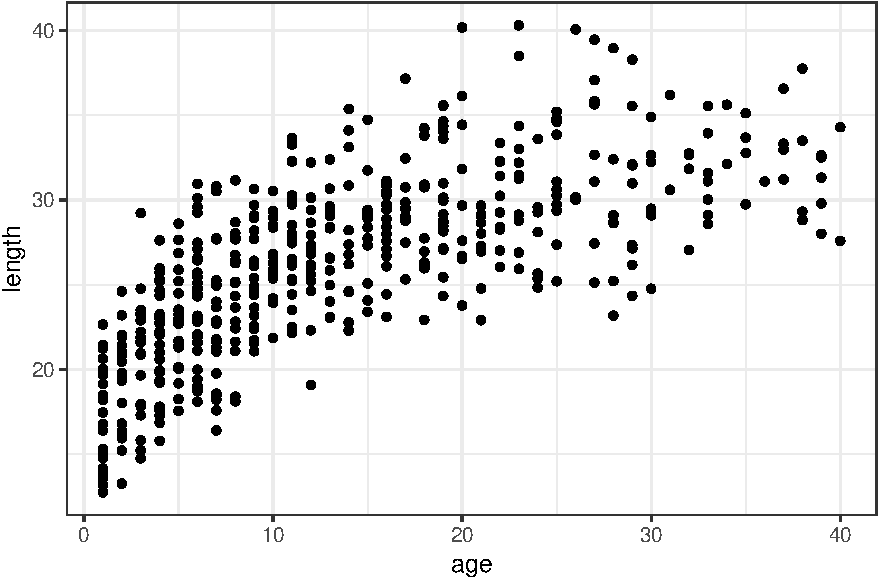
\includegraphics[width=0.7\textwidth]{figures/unnamed-chunk-1-1} \end{center}

\normalsize

\end{frame}

\begin{frame}{Un exemple : relation longueur et âge}

Des données de croisance

Ajustement, `lissage' par la méthode `loess'

\scriptsize

\begin{center}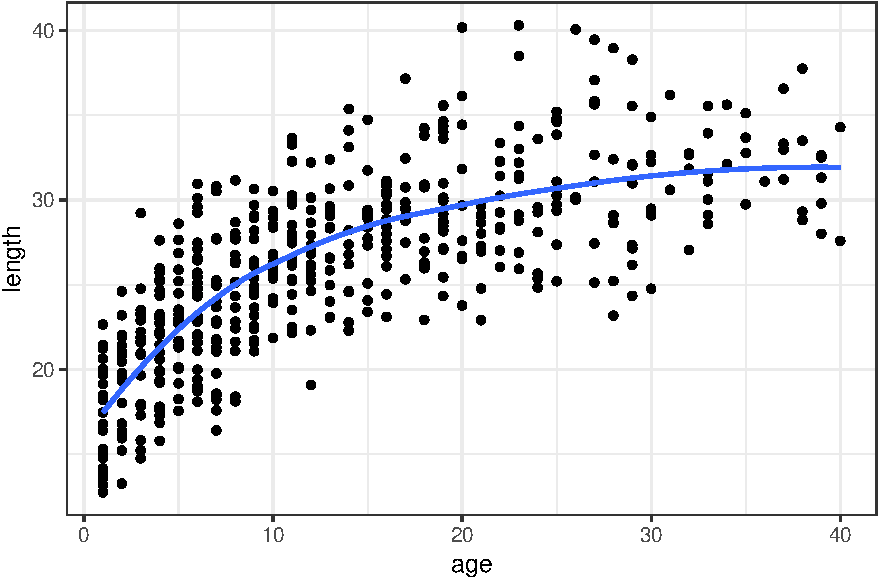
\includegraphics[width=0.7\textwidth]{figures/unnamed-chunk-2-1} \end{center}

\normalsize

On veut représenter le comportement moyen.

\end{frame}

\begin{frame}{Un exemple : relation longueur et âge}

Des données de croisance

Ajustement, `lissage' par la méthode `loess'

\scriptsize

\begin{center}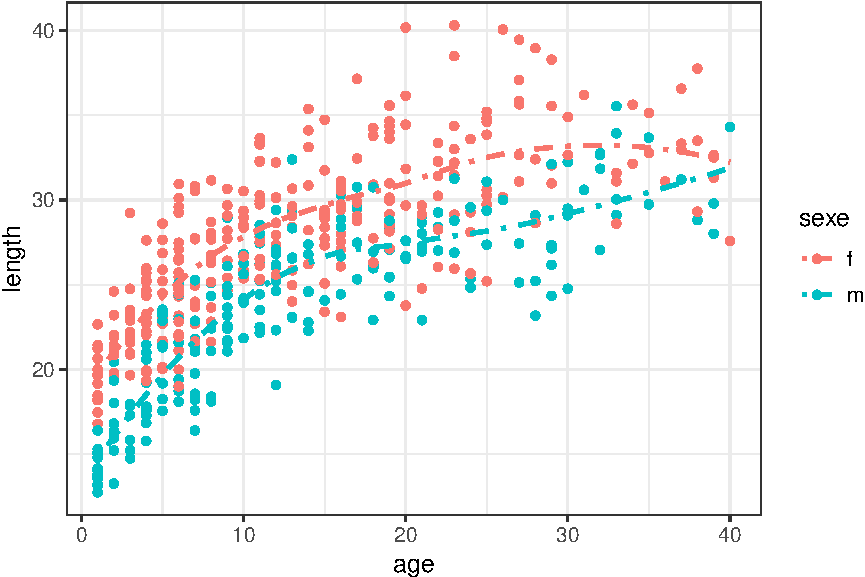
\includegraphics[width=0.7\textwidth]{figures/unnamed-chunk-3-1} \end{center}

\normalsize

On ne peut pas facilement tester si les deux courbes sont
significativement différentes.

\end{frame}

\begin{frame}{Un exemple : relation longueur et âge}

Ajustement d'une relation de von Bertalanffy

\[L_k = L_{\inf} \left ( 1 - e^{ \left \lbrace - K ( x - x_0 ) \right\rbrace } \right) \]

\scriptsize

\begin{center}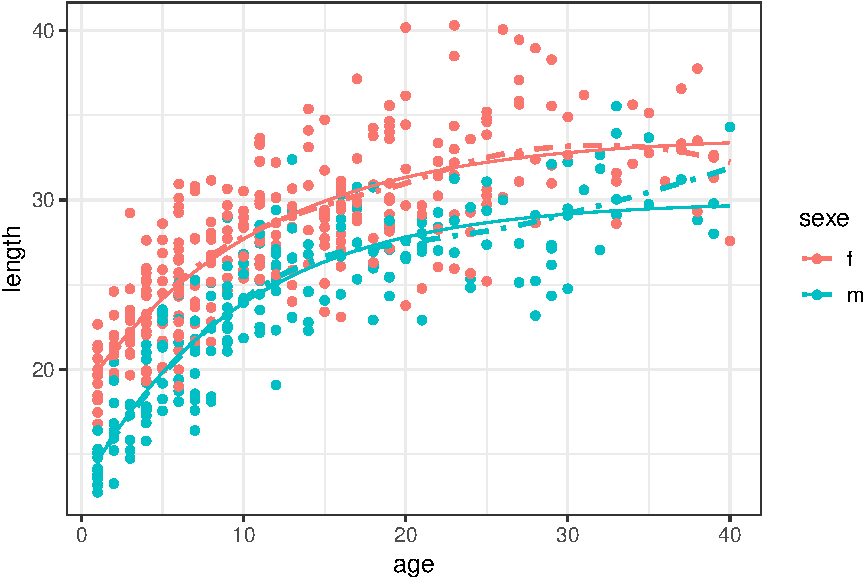
\includegraphics[width=.7\textwidth]{figures/unnamed-chunk-4-1} \end{center}

\normalsize

On a perdu en ajustement mais on peut tester une différence mâle
femelle.

\end{frame}

\begin{frame}[fragile]{Un exemple : relation von Bertalanffy}

\scriptsize

\begin{Shaded}
\begin{Highlighting}[]
\KeywordTok{summary}\NormalTok{(estim_nls)}
\end{Highlighting}
\end{Shaded}

\color{gray}

\begin{verbatim}## 
## Formula: length ~ (ldiff_m * sexe_num + Linf) * (1 - exp(-(kdiff_m * sexe_num + 
##     K) * (age - (xdiff_m * sexe_num + x0))))
## 
## Parameters:
##         Estimate Std. Error t value Pr(>|t|)    
## Linf    33.76311    0.64015  52.743  < 2e-16 ***
## K        0.09158    0.01168   7.838 2.84e-14 ***
## x0      -8.73180    1.28783  -6.780 3.43e-11 ***
## ldiff_m -3.85000    0.88394  -4.355 1.62e-05 ***
## kdiff_m  0.01269    0.01690   0.751   0.4529    
## xdiff_m  3.32673    1.54949   2.147   0.0323 *  
## ---
## Signif. codes:  0 '***' 0.001 '**' 0.01 '*' 0.05 '.' 0.1 ' ' 1
## 
## Residual standard error: 2.752 on 494 degrees of freedom
## 
## Number of iterations to convergence: 10 
## Achieved convergence tolerance: 1.162e-06
\end{verbatim}

\color{black}

\normalsize

\end{frame}

\begin{frame}{Un exemple : relation von Bertalanffy}

\begin{figure}
\centering
\includegraphics{figures/ER_VB.png}
\caption{Fondements vonB - Etienne Rivot}
\end{figure}

\end{frame}

\begin{frame}{Modèle de production de biomasse}

\[B_{t+1} = B_t + g( B_t - C_t),\quad g(b) = \rho b \left (1 - \frac{b}{\kappa}\right)\]

\[B_{MSY} = \frac{\kappa}{2}, \quad C_{MSY} = \frac{\kappa \rho}{4}\]
\scriptsize

\begin{center}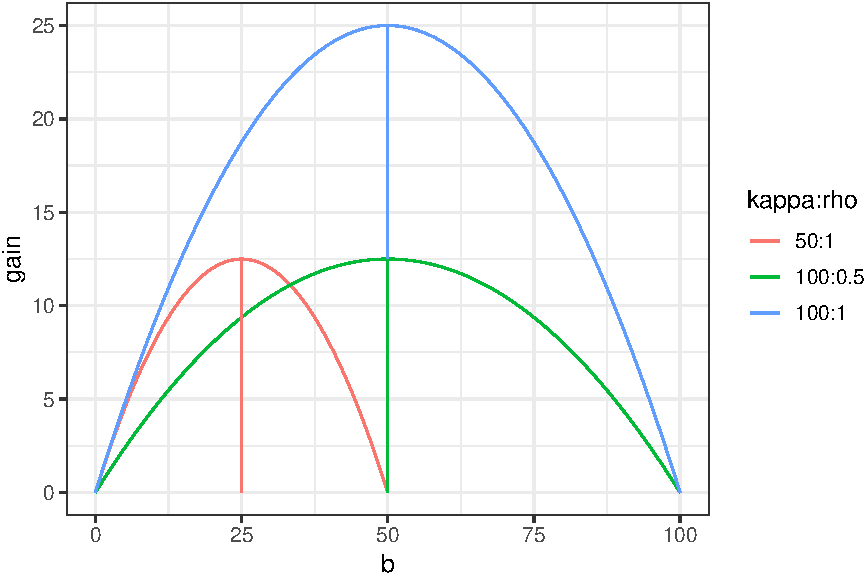
\includegraphics[width=.8\textwidth]{figures/unnamed-chunk-6-1} \end{center}

\normalsize

\end{frame}

\begin{frame}{Des modèles de dynamiques de population - Equations
différentielles}

\begin{figure}
\centering
\includegraphics{figures/ER_Lokta.png}
\caption{Etienne Rivot : Dynamique de population}
\end{figure}

\end{frame}

\begin{frame}{Des modèles écosystémiques - flux}

\begin{figure}
\centering
\includegraphics{figures/ER_ecopath.png}
\caption{Etienne Rivot : Ecopath}
\end{figure}

\end{frame}

\begin{frame}{Des modèles individus centrés}

\begin{figure}
\centering
\includegraphics{figures/ER_IBM.png}
\caption{Etienne Rivot : IBM}
\end{figure}

\end{frame}

\section{Démarche de modélisation}\label{demarche-de-modelisation}

\begin{frame}{Comment se lancer}

\textbf{Il n'existe pas un unique bon modèle qui répond à toutes les
questions}

--

Douglas Adams Le Guide du voyageur galactique :

\emph{Quarante-deux ! cria Loonquawl. Et c'est tout ce que t'as à nous
montrer au bout de sept millions et demi d'années de boulot ?}

\emph{J'ai vérifié très soigneusement, dit l'ordinateur, et c'est
incontestablement la réponse exacte. Je crois que le problème, pour être
tout à fait franc avec vous, est que vous n'avez jamais vraiment bien
saisi la question. }

--

\emph{Essentially, all models are wrong, but some are useful.} (Box,
George E. P.; Norman R. Draper)

\end{frame}

\begin{frame}{Comment se lancer}

\begin{enumerate}
\def\labelenumi{\arabic{enumi}.}
\tightlist
\item
  Définir l'objectif de la modélisation : prédire, comprendre,
\item
  Adopter un principe de parcimonie : choisir le plus petit niveau de
  complexité raisonnable pour répondre à la question.
\end{enumerate}

\end{frame}

\begin{frame}{Le rôle des données}

\begin{itemize}
\tightlist
\item
  Pour émettre des hypothèses
\item
  Pour ajuster le modèle
\item
  Pour tester les qualités du modèle
\end{itemize}

\end{frame}

\begin{frame}{Comment s'y prendre}

\begin{itemize}
\tightlist
\item
  une démarche itérative : on ne construit jamais un modèle en une fois.
\item
  des outils pour estimer les paramètres : MCO, max de vraisemblance
\item
  des outils pour vérifier que le modèle est identifiable (au moins en
  pratique)
\item
  des outils pour juger les qualités prédictives d'un modèle
\end{itemize}

\end{frame}

\begin{frame}{Et maintenant}

\begin{figure}
\centering
\includegraphics{figures/ER_outils.png}
\caption{Etienne Rivot : conclusions}
\end{figure}

\end{frame}

\end{document}
